%qqqqqqqqqqqqqqqqqqqqqqqqqqqqqqqqqqqqqqqqqqqqqqqqqqqqqqqqqqqqqqqqqqqqqqqqq
%Quote
\begin{savequote}[50mm]
‘‘The Cosmos is all that is or was or ever will be. Our feeblest contemplations 
of the Cosmos stir us: there is a tingling in the spine, a catch in the voice, 
a faint sensation, as if a distant memory, of falling from a height. We know 
we are approaching the greatest of mysteries’’

\qauthor{Carl Sagan}
\end{savequote}
%qqqqqqqqqqqqqqqqqqqqqqqqqqqqqqqqqqqqqqqqqqqqqqqqqqqqqqqqqqqqqqqqqqqqqqqqq




%#########################################################################
\chapter{Theoretical Framework in Cosmology}
\label{cha:Theoretical Framework}


%Reviewed
The aim of this chapter is to cover, in a self-contained and summarized 
way, all the theoretical framework needed for the study of the large-scale
universe. From the simplest models of the universe given by Friedman's 
solutions, the theory of perturbations for the formation of complex 
structures like galaxies and galaxy clusters, until the schemes to 
quantify the cosmic web.



%#########################################################################




%*************************************************************************
%Isotropic and homogeneous universe
\section{Isotropic and Homogeneous Universe}
\label{sec:IsotropicAndHomogeneousUniverse}


%Reviewed
The two big pillars of the modern cosmology are the cosmological principle
and the theory of the general relativity. The first one is a principle 
where it is assumed that the universe is isotropic and homogeneous at very
large scales, while the second one gives the theoretical support needed in 
order to understand properly the relation between the matter content of 
the universe and the structure of the space-time.


%Reviewed
As it has been evidenced by observations of large-scale structures and the 
CMB, the universe appears to be isotropic and homogeneous at large scales,
which is in agreement with the cosmological principle. Moreover, this fact
simplifies quite enough the complex tensorial formulation of the general
relativity, thereby allowing finally leading to the Friedmann's equations.



	%---------------------------------------------------------------------
	%Curved space metric
	\subsection{Metric of Curved Spaces}
	\label{subsec:MetricOFCurvedSpaces}
	%---------------------------------------------------------------------

	
%Reviewed
In the construction of an isotropic and homogeneous model of universe, it 
is necessary to establish an adequate metric which describes it properly. 
An illustrative example that could be generalized is a 2D spherical 
surface, which clearly satisfies the criteria of homogeneity and isotropy.



%.........................................................................
%2D sphere
\begin{figure}[htbp]
	\centering
	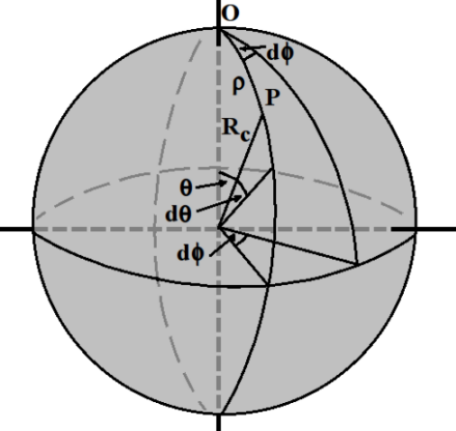
\includegraphics[width=0.5\textwidth]
	{./figures/2_theoretical_framework/2D_Sphere.png}
	
	\caption{\small{Metric of a spherical surface.}}
	
	\label{fig:2sphere}
\end{figure}
%.........................................................................


%Reviewed
A line element over the surface shown in Figure \ref{fig:2sphere} can
be described as


%Reviewed
%.........................................................................
%Line element on the sphere
\[ dl^2 = d\rho^2 + R_c^2 \sin^2 \pr{ \frac{\rho}{R_c}}d\phi^2 \]
%.........................................................................
where it have been introduced a new length coordinate over the surface, 
defined as $\rho = \theta R_c$ and $R_c$ is the curvature radius of the 
sphere. Another very convenient way to rewrite this expression, and that 
allowing a very useful generalization, it is reached defining the curvature
parameter $k$ and the coordinate $r = \sin (\rho/a)$, obtaining:


%Reviewed
%.........................................................................
%Line element on the sphere with time-dependent curvature
\[ dl^2 = a^2(t) \cor { \frac{dr^2}{1-kr^2} + r^2 d\phi^2 } \]
%.........................................................................
with $k = -1$ and it is assumed a time-dependent curvature radius $R_c = 
a(t)$. The metric in this case is 3D and is obtained by replacing the 
differential element of angle $d\phi^2$ by the solid angle differential 
$d\Omega^2 = d\theta^2 + \sin^2\theta d\phi^2$.


 
%.........................................................................
%Line element on the 3-sphere
\eq{eq:LineElement3D}
{ dl^2 = a^2(t) \cor { \frac{dr^2}{1-kr^2} + r^2 (d\theta^2 + 
\sin^2\theta d\phi^2)} }
%.........................................................................


%Reviewed
Finally, time is included, so the space-time interval for the metric of
isotropic and homogeneous curved spaces is:



%.........................................................................
%Interval element on the 3-sphere
\eq{eq:IntervalCurvedSpaces}
{ ds^2 = c^2 dt^2 - a^2(t) \cor { \frac{dr^2}{1-kr^2} + r^2 (d\theta^2 + 
\sin^2\theta d\phi^2)} }
%.........................................................................


%Reviewed
The direct generalization of this expression consists in varying the 
different values of the curvature parameter $k$ in order to obtain the 
metric of flat ($k = 0$), spherical closed ($k = -1$) or opened spaces
($k = 1$), as it is shown in \cite{longair2008} or \cite{padmanabhan1995}.


\
%.........................................................................
%Curved Spaces
\begin{figure}[htbp]
	\centering
	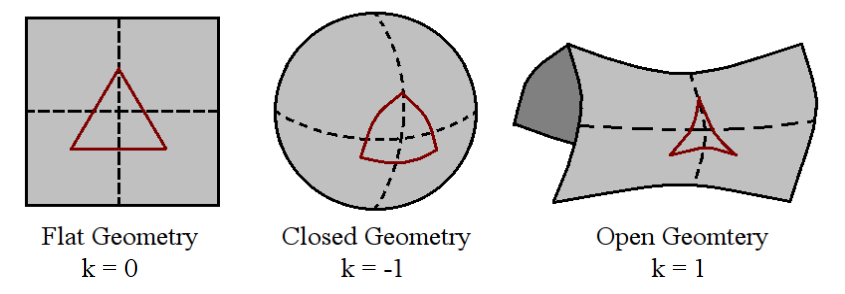
\includegraphics[width=0.9\textwidth]
	{./figures/2_theoretical_framework/Curved_Spaces.png}

	\caption{\small{Curved spaces according to the curvature parameter.}}
	
	\label{fig:CurvedSpaces}
\end{figure}
%.........................................................................
\

%Reviewed
An alternative way to rewrite the metric is introducing two changes of 
coordinates defined as



%.........................................................................
%Xi variable
\[ \chi = \int \frac{ dr'}{\sqrt{1 - k r'^2}}\]
%.........................................................................


%Reviewed
%.........................................................................
%Proper time
\[ \tau = \int \frac{ c dt'}{a(t')}\]
%.........................................................................
where each one is respectively interpreted as a length coordinate over the 
hypersurface that defines the space ($\chi$) and as the proper time 
measured locally ($\tau$). It is obtained the next expressions for the 
metric



%.........................................................................
%Interval element generalized
\eq{eq:IntervalCurvedSpacesAltern1}
{ ds^2 = c^2 dt^2 - a^2(t) \cor { d\xi^2 +  f^2_k(\xi)(d\theta^2 + 
\sin^2\theta d\phi^2)} }
%.........................................................................


%Reviewed
%.........................................................................
%Interval element generalized
\eq{eq:IntervalCurvedSpacesAltern2}
{ ds^2 = \bar a^2 (\tau)\cor{ d\tau^2 - d\xi^2 -  f^2_k(\xi)(d\theta^2 + 
\sin^2\theta d\phi^2)} }
%.........................................................................
where the function $f_k(\chi)$ is defined according to the value of the 
curvature parameter.



%.........................................................................
%Curvature Function
\eq{eq:CurvatureFunction}
{ f_k(\chi) = \left\{  \matrix{	
\sin \chi	&	k = 1		\cr 
\chi 		& 	k = 0 		\cr	
\sinh \chi 	& 	k = -1 		\cr } \right.  }
%.........................................................................


%Reviewed
In spite of the derived expressions for the metric 
\ref{eq:IntervalCurvedSpaces} \ref{eq:IntervalCurvedSpacesAltern1} and
\ref{eq:IntervalCurvedSpacesAltern2} are completely equivalent, the usage
of one or another depends on the specific problem. Specially the 
expression \ref{eq:IntervalCurvedSpacesAltern1} is usually more used and
is defined as the Friedmann's metric.


%Reviewed
It could be shown that in Riemannian manifolds \footnote{A Riemannian 
manifold is a space where it can be defined (well-defined) a metric.},
the space-time interval is expressed in terms of the metric tensor as
\cite{weinberg1972}


%Reviewed
%.........................................................................
%Metric-Interval relation
\[ ds^2 = g_{\mu \nu}dx^\mu dx_\nu \]
%.........................................................................
where it has been introduced the cuadrivector $x^\mu = 
(ct, r, \theta, \phi)$.


%Reviewed
Due to the assumption of isotropy and homogeneity, the metric tensor must
be diagonal, furthermore, comparing with the expression 
\ref{eq:IntervalCurvedSpaces}, it is possible to obtain the next explicit 
form



%.........................................................................
%MetricTensor
\eq{eq:MetricTensor}
{g_{\mu \nu} = \pr{ \matrix{ 
1		&				0			&		0			&				0				\cr
0		&	-a^2(t)(1 - kr^2)^{-1}	&	 	0			&				0				\cr
0		&				0			&	-a^2(t)r^2		&				0				\cr
0		&				0			&		0			&	-a^2(t)r^2 \sin^2 \theta } }}
%.........................................................................


%Reviewed
From this metric and the Einstein's field equations, it is possible to 
build simple models of the universe, such as it shall be shown in the 
subsection \ref{subsec:GeneralRelativityAndFriedmannEquations}.



			%-------------------------------------------------------------
			%Measuring distances
			\subsubsection*{Measuring Distances}
			%-------------------------------------------------------------


%Reviewed
Once defined the metric of curved spaces, it is very useful to introduce
some concepts related with distances, which are used recurrently 
\cite{longair2008}. For the sake of simplicity it will be assumed a flat 
metric ($k = 0$).


%Reviewed
\begin{itemize}
%Comovil Radial Distance..................................................
\item \textit{\textbf{Comoving radial distance:}} by definition, a light
signal has an associated null interval, i.e. $ds^2 = 0$. Using the 
expression \ref{eq:IntervalCurvedSpaces} for the metric, it is obtained


%Reviewed
%.........................................................................
%Comovil Distance
\eq{eq:ComovilDistance}
{ r = \int_t^{t_0} \frac{ cdt'}{a(t')} = \int_a ^1 \frac{ c da}{a \dot a} }
%.........................................................................
where the specific form of $a(t)$ depends on the specific chosen cosmology
(see subsection \ref{subsec:SimpleSolutionsOfTheUniverse}) and $t_0$ is the
reference time, which is taken as the current age of the universe.


%Reviewed
Due to the assumption of an expanding metric, the distance between two 
objects depends on the time in which the measurement is performed. 
Moreover, the distance cannot be determined from a beam of light since
light has a finite velocity \footnote{$c=299\ 792\ 458$ m/s}. Because of 
that, it must be performed a projection on the light-cone traced by the 
beam in the current time, such as it is made in the expression 
\ref{eq:ComovilDistance}. The latter allows interpreting $r$ as the 
distance to an object in the current time, and it is quite different to
the apparent distance which corresponds to the time when the object in 
question emitted the observed light.


%Reviewed
%Proper Radial Distance..................................................
\item \textit{\textbf{Proper radial distance:}} by virtue of the 
definition of scale factor, to obtain the distance to an object in any 
time, it is enough to multiply the comoving distance by the scale factor 
evaluated in the same time, that is



%.........................................................................
%Proper Distance
\eq{eq:ComovilDistance}
{ r_{\submath{prop}} = a(t)\int_t^{t_0} \frac{ cdt'}{a(t')} = 
a\int_a ^1 \frac{ c da}{a \dot a} }
%.........................................................................	


%Reviewed
%Particle Horizon........................................................
\item \textit{\textbf{Particle horizon:}} considering a beam travelling 
through vacuum since the beginning of all time, at $t=0$; the maxim proper
distance that could be travelled by the light in a time $t$ is denominated 
particle horizon and determines all regions in the universe that could 
have been causally connected in that time. 



%.........................................................................
%Particle Horizon distance
\eq{eq:HorizonDistance}
{ r_{\submath{H}} = a(t)\int_0^{t} \frac{ cdt'}{a(t')} = 
a\int_0 ^a \frac{ c da}{a \dot a} }
%.........................................................................

\end{itemize}
	%---------------------------------------------------------------------
	%General relativity and Friedmann equations
	\subsection{General Relativity and Friedmann's Equations}
	\label{subsec:GeneralRelativityAndFriedmannEquations}
	%---------------------------------------------------------------------
	

%Reviewed
The Einstein's field equations of the general relativity play a fundamental
role since they express explicitly the relation between the matter 
content of the universe and the local geometry of the space-time.


%Reviewed
%.........................................................................
%EinsteinEquations
\eq{eq:EinsteinEquations}
{ R_{\mu \nu} - \frac{1}{2}R - g_{\mu \nu}\Lambda = 
\frac{8\pi G}{c^4}T_{\mu \nu} }
%.........................................................................
or equivalently


%Reviewed
%.........................................................................
%Einstein Equations Alternative
\eq{eq:EinsteinEquationsAltern}
{ R_{\mu \nu} + g_{\mu \nu}\Lambda = 
\frac{8\pi G}{c^4}\pr{T_{\mu \nu} - \frac{1}{2}T g_{\mu \nu}} }
%.........................................................................
where $T$ is the trace of the energy-momentum tensor (see 
\ref{eq:MomentumEnergyTensor}), $R_{\mu \nu}$ the Ricci curvature tensor
and $R$ the scalar curvature. The last two terms are calculated from 
different traces of the Riemann curvature tensor, as $R_{\mu \nu} = 
R^\eta_{\ \mu \eta \nu}$ and $R = R^{\mu}_{\ \mu}$. For convenience, it
has been introduced the term associated with the cosmological constant, 
which will be used below to calculate different models of the universe 
with dark energy contribution.


%Reviewed
The Riemann curvature tensor quantifies deviations of the metric of curved 
space-times with respect to the Euclidean metric and allows to determinate
completely the geometrical properties like the local curvature, different 
measures of distances and angles, etc. \cite{weinberg1972}. This tensor is
built from the Levi-Civita connection as


%Reviewed
%.........................................................................
%Riemann Tensor
\eq{eq:RiemannTensor}
{ R^\mu_{\ \nu \alpha \beta} = 
\Gamma^\mu_{\ \nu \alpha, \beta} -  
\Gamma^\mu_{\ \nu \beta, \alpha} + 
\Gamma^\mu_{\ \sigma \alpha}\Gamma^\sigma_{\ \nu \beta}-
\Gamma^\mu_{\ \sigma \beta}\Gamma^\alpha_{\ \nu \alpha}}
%.........................................................................
with the Levi-Civita connection defined from the metric as



%.........................................................................
%Afin Connection
\eq{eq:AfinConnection}
{ \Gamma^\nu _{\ \alpha \beta}  = \frac{1}{2}g^{\mu \sigma}
\pr{ g_{\sigma \alpha, \beta} + g_{\sigma \beta, \alpha} -
g_{\alpha \beta, \sigma} } }
%.........................................................................


%Reviewed
The right-hand side of the equation \ref{eq:EinsteinEquations} contains
the energy-momentum tensor $T_{\mu \nu}$, which characterizes the density
and the matter-energy flux of the universe. By virtue of the cosmological 
principle, this tensor must also be diagonal and if, furthermore, it is 
assumed an ideal fluid model, the next form is obtained



%.........................................................................
%MomentumEnergyTensor
\eq{eq:MomentumEnergyTensor}
{T^\mu_{\ \nu} = \pr{ \matrix{ 
c\rho^2	&	0	&	0	&	0				\cr
0		&	-P	&	0	&	0				\cr
0		&	0	&	-P	&	0				\cr
0		&	0	&	0	&	-P } }}
%.........................................................................


%Reviewed
Finally, using the equations \ref{eq:MetricTensor}, 
\ref{eq:EinsteinEquationsAltern} and \ref{eq:MomentumEnergyTensor}, it is 
possible to reduce the complex system of tensorial equations to two scalar
coupled equations which are usually called Friedmann's equations 
\cite{longair2008}. These equations describe completely the evolution of
an isotropic and homogeneous universe in terms of the scale factor $a(t)$ 
(see equation \ref{eq:LineElement3D})



%.........................................................................
%Friedmann Equation 1
\eq{eq:FriedmannEquation1}
{ \frac{\ddot a}{a} = -\frac{4\pi G}{3}\pr{\rho + \frac{3P}{c^2}}
+ \frac{c^2 \Lambda}{3}}
%.........................................................................


%.........................................................................
%Friedmann Equation 2
\eq{eq:FriedmannEquation2}
{ \frac{\ddot a}{a} + 2\frac{\dot a^2}{a^2} + 2\frac{c^2 k}{a^2} =
4\pi G \pr{ \rho - \frac{P}{c^2} } + c^2 \Lambda}
%.........................................................................


%Reviewed
In order to solve this equation system in terms of $a(t)$ and thereby 
obtaining the evolution of the scale factor, it is necessary to know the 
explicit time-dependent expression of the density $\rho$ and the pressure
$P$, or equivalently, the dependence on the scale factor. This must be done
for each type of energy-matter of the universe. A detailed derivation of
these explicit expressions could be found in \cite{longair2008} and they
are summarized in Table \ref{tab:PropertiesDependence}.



%.........................................................................
%Table of dependences of Matter-Energy content of the universe with a
\begin{table}[htbp]
\centering
\begin{tabular}{|c|c|c|c|} \hline
\cellc{\textbf{Property}} 	& 
\cellc{\textbf{Density}} 	&
\cellc{ \textbf{Pressure}}	& 
\cellc{\textbf{Temperature}}		\\ \hline

& & &  \\
\textbf{Matter}& $\rho = \rho_0 a^{-3}(t)$ & $p = p_0 a^{-5}(t)$ & $T = T_0 a^{-2}(t)$ \\ 
\small{(baryonic + dark)} & & &  \\ \hline
& & &  \\
\textbf{Radiation }& $\rho = \rho_0 a^{-4}(t)$ & $p = p_0 a^{-4}(t)$ & $T = T_0 a^{-1}(t)$ \\ 
\small{(+ relativistic matter)} & & &  \\ \hline
& & &  \\
\textbf{Vacuum }& $\rho = \rho_0 $ & $p = p_0 $ & $-$ \\ 
& & &  \\ \hline
\end{tabular}
\caption{Dependence of some quantities on the scale factor $a(t)$
\cite{longair2008}.}
\label{tab:PropertiesDependence}
\end{table}
%.........................................................................


%Reviewed
By convention, it has been taken the current scale factor as $a_0 = a(t_0) 
= 1$ and the reference values are defined as $\rho_0 = \rho(a_0)$, $P_0 = 
P(a_0)$ and $T_0 = T(a_0)$. Using the Friedmann's equations, defining the
Hubble parameter as $H(t) = \dot a/ a$ and the vacuum density as 
$\rho_\Lambda = c^2\Lambda/8\pi G$, it is obtained



%.........................................................................
%Pre Hubble Equation
\[ \pr{ \frac{\dot a}{a} }^2 = H^2(t) = \frac{ 8\pi G}{3}
\cor{ \rho_{m}\frac{1}{a^{3}} + \rho_{r}\frac{1}{a^{4}} + \rho_{\Lambda} }
- \frac{ c^2 k }{a^2} \]
%.........................................................................


%Reviewed
Evaluating this expression in the current epoch $H(t_0) = H_0$, with $H_0$
the Hubble constant and defining the critical density $\rho_c$ as the 
density that the universe must have in order to be flat.


%Reviewed
%.........................................................................
%Critical Density
\eq{eq:CriticalDensity}
{ \rho_c = \frac{3H_0^2}{8\pi G} }
%.........................................................................
it leads to the equation of evolution for the Hubble parameter


%Reviewed
%.........................................................................
%Hubble Equation
\eq{eq:HubbleEquation}
{ H^2(t) = H_0^2 \cor{ 
(1 - \Omega_0)\frac{1}{a^2} +  
\Omega_m \frac{1}{a^3} +
\Omega_r \frac{1}{a^4} +
\Omega_\Lambda} }
%.........................................................................
where it has been introduced the density parameters $\Omega_i$, defined
as the current density of the i-th specie in the current epoch, normalized 
with the critical density \ref{eq:CriticalDensity}, and $\Omega_0 = 
\sum_i \Omega_i$. These density parameters along with the Hubble constant
are part of the free parameters of the theory and must be determined by 
observations. This allows to characterize different particular cosmologies
\footnote{\textit{Cosmology} must be understood in this context as a 
specific solution of the Friedmann's equations.}



	%---------------------------------------------------------------------
	%Simple solutions of the universe
	\subsection{Simple Solutions of the Universe}
	\label{subsec:SimpleSolutionsOfTheUniverse}
	%---------------------------------------------------------------------


%Reviewed
Although in this stage it has not been introduced the complete formalism 
of small perturbations and structure formation, the set of equations
\ref{eq:FriedmannEquation1}, \ref{eq:FriedmannEquation2} and 
\ref{eq:HubbleEquation} leads to a first and rough understanding of the
evolution of the Universe.


%Reviewed
In this subsection, it will be presented some analytic solutions to the 
Friedmann's equations. In spite of the ideal assumptions on which are
based, in some cases, they can be used as approximations in some stages
of evolution of the universe, thus allowing a physical understanding more 
adequate than exact numerical solutions.



			%-------------------------------------------------------------
			%Einstein-de Sitter Universe
			\subsubsection*{Einstein - de Sitter Universe}
			%-------------------------------------------------------------


%Reviewed
The Einstein-de Sitter Universe is a cosmological model with a flat metric
and composed entirely of matter, this implies that $\Omega_0 = \Omega_m = 1$ 
and $k=0$. Applying this in equation \ref{eq:HubbleEquation}, it is obtained
the next expression



%.........................................................................
%EinsteindeSitter
\eq{eq:EinsteindeSitter}
{ H^2(t) = \pr{\frac{\dot a}{a}}^2 = H_0^2 \frac{1}{a^3} }
%.........................................................................


%Reviewed
Integrating, it leads to the explicit time-dependent solution for the 
scale factor



%.........................................................................
%EinsteindeSitterSolution
\eq{eq:EinsteindeSitterSolution}
{ t(a) = \frac{ 2}{3H_0} a ^{3/2} }
%.........................................................................


%Reviewed
Although in this case it is possible to obtain the explicit form of $a(t)$,
most of the time it is only possible to have the implicit solution $t(a)$.
Another very useful way to describe this solution is by using the redshift
$z$, which is related with the scale factor as \cite{longair2008}


%Reviewed
%.........................................................................
%Redshift
\eq{eq:Redshift}
{ z + 1 = \frac{ a_0}{a} }
%.........................................................................
to finally obtain



%.........................................................................
%EinsteindeSitterSolutionZ
\eq{eq:EinsteindeSitterSolutionZ}
{ t(a) = \frac{ 2}{3H_0} (1+z) ^{-3/2} }
%.........................................................................


%Reviewed
This solution is quite close to the real behaviour of the universe in the 
matter-dominated epoch, between $70000$ and $5$ millions of years after 
the Big Bang \cite{padmanabhan1995}.



			%-------------------------------------------------------------
			%Radiation Dominated Universe
			\subsubsection*{Radiation-Dominated Universe}
			%-------------------------------------------------------------


%Reviewed
In this case, it will be assumed that the universe is radiation-dominated, 
that is $\Omega_0 = \Omega_r$, but not necessarily flat. The Friedmann's 
equations lead to the next expression



%.........................................................................
%Radiation Universe
\eq{eq:RadiationUniverse}
{ H^2(t) = \pr{\frac{\dot a}{a}}^2 = H_0^2 \cor{ 
(1 - \Omega_r)\frac{1}{a^2} +  \Omega_r \frac{1}{a^4}} }
%.........................................................................


%Reviewed
Integrating this expression, it is obtained the next implicit solution for
the scale factor


%Reviewed
%.........................................................................
%Radiation Universe Solution
\eq{eq:RadiationUniverseSolution}
{ t = \left\{  \matrix{ 
H_0^{-1}(\Omega_r - 1)^{-1}\pr{ \Omega_r^{1/2} - 
\cor{a^2(1-\Omega_r) + \Omega_r}^{1/2} } & \Omega_r \neq 1 \cr
H_0^{-1} a^2/2 & \Omega_r = 1} \right. }
%.........................................................................
or in terms of redshift



%.........................................................................
%Radiation Universe Solution Z
\eq{eq:RadiationUniverseSolutionZ}
{ t = \left\{  \matrix{ 
H_0^{-1}(\Omega_r - 1)^{-1}\pr{ \Omega_r^{1/2} - 
\cor{(1+z)^{-2}(1-\Omega_r) + \Omega_r}^{1/2} } & \Omega_r \neq 1 \cr
H_0^{-1} (1+z)^{-2}/2 & \Omega_r = 1} \right. }
%.........................................................................


%Reviewed
This solution is useful as an approximation for the radiation-dominated 
epoch, which happened from the big bang until the recombination epoch, 
approximately $380 000$ years after the big bang, or equivalently in a
redshift of $z = 1100$ \cite{padmanabhan1995}.



			%-------------------------------------------------------------
			%Vacuum Dominated Universe
			\subsubsection*{Vacuum-dominated Universe}
			%-------------------------------------------------------------
		

%Reviewed	
This type of hypothetical universe is completely vacuum-dominated, or
equivalently dominated by the cosmological constant. Making $\Omega_0 = 
\Omega_\Lambda$ in the Friedmann's equations, it is obtained
			


%.........................................................................
%Vacuum Universe
\eq{eq:VacuumUniverse}
{ H^2(t) = \pr{\frac{\dot a}{a}}^2 = H_0^2 \cor{ 
(1 - \Omega_\Lambda)\frac{1}{a^2} +  \Omega_\Lambda} }
%.........................................................................


%Reviewed	
Solving for $t(a)$


%Reviewed
%.........................................................................
%Vacuum Universe Solution
\eq{eq:VacuumUniverseSolution}
{ t = \frac{1}{H_0^2 \Omega_\Lambda^{1/2}}
\ln\cor{ a \pr{ \frac{\Omega_\Lambda}{1 - \Omega_\Lambda} }^{1/2} +
\pr{ 1 + \frac{\Omega_\Lambda}{1 - \Omega_\Lambda}a^2 }^{1/2} } }
%.........................................................................
and using the redshift



%.........................................................................
%Vacuum Universe Solution Z
\eq{eq:VacuumUniverseSolutionZ}
{ t = \frac{1}{H_0^2 \Omega_\Lambda^{1/2}}
\ln\cor{ \frac{1}{1+z} \pr{ \frac{\Omega_\Lambda}{1 - \Omega_\Lambda} }^{1/2} +
\pr{ 1 + \frac{\Omega_\Lambda}{1 - \Omega_\Lambda}\frac{1}{\pr{1+z}}^2 }^{1/2} } }
%.........................................................................


%Reviewed
This solution is very interesting because, unlike the previous solutions, 
is only valid for values of the density parameter within the range 
$0<\Omega_\Lambda <1$. This implies that it is not possible to have a  
universe with flat or hyperbolic geometry when it is vacuum-dominated.
Another aspect equally remarkable is the concavity of the scale factor 
$a(t)$ obtained from \ref{eq:VacuumUniverseSolution} (see Figure 
\ref{fig:Cosmologies}), which shows an accelerated expansion of the 
universe. This characteristic is only possible when there is a non-null 
term associated to the vacuum energy.


%Reviewed
Finally and like the previous solutions, the expression 
\ref{eq:VacuumUniverseSolution} can be used as an approximation for the
vacuum-dominated epoch of the universe, which lasts from the end of the
matter-dominated epoch, $5$ millions of years after the big bang, until 
nowadays \cite{longair2008}.



			%-------------------------------------------------------------
			%WMAP7 Universe
			\subsubsection*{WMAP7 Universe}
			%-------------------------------------------------------------
			
			
%Reviewed
The set of parameters associated to the standard cosmological model has 
been measured on several occasions by different spacecraft missions (see
section \ref{sec:CosmologicalObservations}). Among those measurements it 
is notable the one conducted by WMAP. The data obtained after seven years
of observation (WMAP7) are adopted in this work \cite{WMAP7}. Among the 
cosmological parameters measured are the Hubble constant and the density
parameters $\Omega_i$. Taking the values given in Table 
\ref{tab:CosmologicalParameters} and for simplicity assuming $\Omega_0 = 1$
it is possible to integrate the Friedmann's equations

			
%Reviewed	
%.........................................................................
%WMAP Universe
\eq{eq:WMAPUniverse}
{ H^2(t) = H_0^2 \cor{ 
\Omega_m \frac{1}{a^3} +
\Omega_r \frac{1}{a^4} +
\Omega_\Lambda} }
%.........................................................................
to obtain


%.........................................................................
%WMAP Universe
\eq{eq:WMAPUniverse}
{ t = \frac{1}{H_0}\int _0 ^{a}\cor{ 
\Omega_m \frac{1}{a'} + 
\Omega_r \frac{1}{a'^2} +
\Omega_\Lambda a'^2 }^{-1/2}da' }
%.........................................................................

\
%.........................................................................
%Friedmann Solutions
\begin{figure}[htbp]
	\centering
	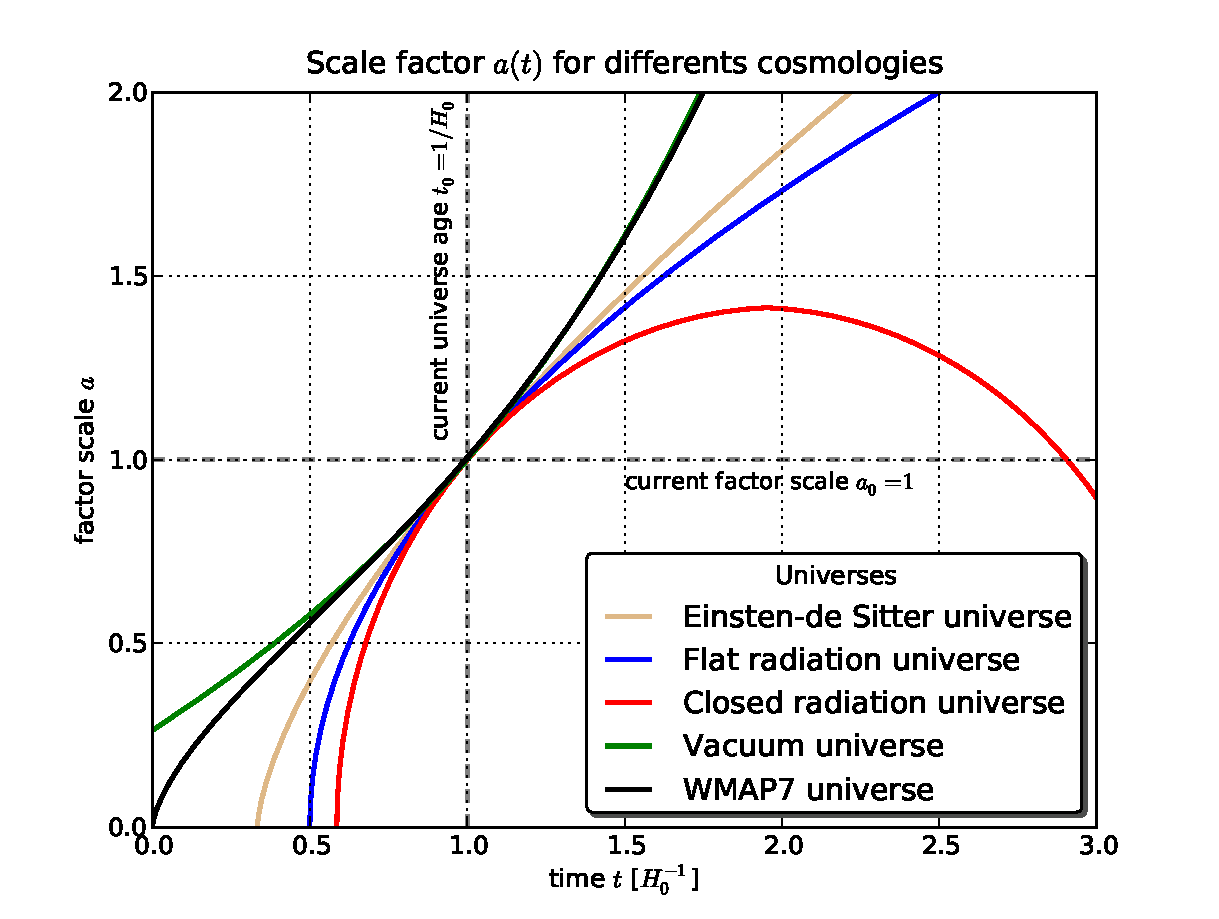
\includegraphics[width=0.9\textwidth]
	{./figures/2_theoretical_framework/Friedmann_Solution.pdf}

	\caption{\small{Different solutions of the universe according to the
	Friedmann's equations.}}
	
	\label{fig:Cosmologies}
\end{figure}
%.........................................................................
\

%Reviewed
It is possible to obtain an analytic solution of this integral in terms of
elliptic functions, but for simplicity it is chosen the numerical solution.
In Figure \ref{fig:Cosmologies} is shown the solution for a WMAP7 
universe and it is compared to other cosmologies, derived previously.


%Reviewed
An interesting characteristic of the solution for the WMAP7 universe is 
the change of concavity (black curve in Figure \ref{fig:Cosmologies}), 
which indicates a transition from the matter/radiation-dominated epoch
to an accelerated expanding regime associated to the vacuum energy.
Another important aspect is the prediction of the age of the universe.
Taking into account the previously defined normalization for the scale
factor $a(t_0) = a_0$, it is straightforward to see that $t_0 = H_0^{-1} 
\approx 13.75 \times 10^9$ years. Other cosmologies under the same 
normalization predict different ages, since larger values such as a 
vacuum-dominated universe, until smaller and even a collapse time (usually
known as big crunch time) such as a radiation-dominated and closed 
universe.



%*************************************************************************




%*************************************************************************
%Linear Structure Formation
\section{Linear Regime of Structure Formation}
\label{sec:LinearStructureFormation}


%Reviewed
The previous section deals about the universe as a whole, assuming as 
valid the condition of isotropy and homogeneity. Although the real universe
has this asymptotic behaviour at very large scales, at smaller local scales
the behaviour is quite different, being even completely anisotropic and 
highly non-homogeneous. Life is certainly the most illustrative example of 
that, one of the highest non-linearities of the universe, and thus, 
planets, stars, galaxies, galaxy clusters, in the same decreasing order of 
inhomogeneity and anisotropy.


%Reviewed
The standard way to introduce these local structures in the universe is by
assuming as valid the solutions of the Friedmann's equations at very large 
scales, but considering inhomogeneities as perturbations of the model. 
First, in the linear regime, where the perturbations in the density field
are much smaller than the background mean density ($\delta \rho \ll 
\rho_b$), and after, in the non-linear regime, where the perturbations are
comparable or even larger ($\delta \rho \sim \rho_b$) (see section 
\ref{sec:NonLinearStructureFormation}).

 

	%---------------------------------------------------------------------
	%Newtonian Approximation
	\subsection{Newtonian Approximation}
	\label{subsec:Newtonian Approximation}
	%---------------------------------------------------------------------


%Reviewed
The frame of linear evolution can be presented in two ways. The first 
one is by considering a perturbative term in the energy-momentum tensor
$ \delta T_{\mu \nu}$ and linearizing the Einstein's field equations 
\ref{eq:EinsteinEquations} and finally solving for $\delta R_{\mu \nu}$



%.........................................................................
%Perturbative Einstein Equations
\eq{eq:PerturbativeEinsteinEquations}
{ \mathcal{L}( R_{\mu \nu}, \delta R_{\mu \nu} ) = 
\frac{8\pi G}{c^2}\pr{ T_{\mu \nu} + \delta T_{\mu \nu} } }
%.........................................................................


%Reviewed
Although this method is, rigorously, more adequate, it has an inconvenience
which makes it very complicated of applying. Non-perturbative terms are 
not necessarily small in all the coordinate systems, inclusively, they can 
reach values with the same order or even bigger than the background mean 
density \cite{padmanabhan1995}.


%Reviewed
The second method consists in assuming perturbations with a comoving size
smaller than the Hubble radius ($r_\delta \ll r_H \sim cH_0^{-1}$)
\footnote{The Hubble radius $r_H$ is a length unit that defines the 
order of magnitude of the size of the observable universe.}, thereby
being possible to neglect relativistic effects due to the curvature
of the space-time. Once this is done, it is possible to use a Newtonian
scheme to evolve perturbations of the background universe. This scheme
assumes that the matter content of the universe is a fluid described by
three basic equations of fluid mechanics. The first one is the continuity
equation, which expresses mass conservation in a fluid



%.........................................................................
%Continuity equation
\eq{eq:ContinuityEquation}
{ \dtot{\rho}{t} = - \rho \nabla \cdot \bds u }
%.........................................................................


%Reviewed
The second one, Euler's equation, characterizes the velocity field of the 
fluid, and physically it expresses the momentum conservation law


%.........................................................................
%Euler Equation
\eq{eq:EulerEquation}
{ \dtot{\bds u}{t} = -\frac{ \nabla P}{\rho} - \nabla \varphi }
%.........................................................................


%Reviewed
And finally the Poisson's equation, which is the non-relativistic version
of the Einstein's field equations and expresses the relation between the
matter content of the universe and sources of gravitational field.

	
	
%.........................................................................	
%Poisson Equation
\eq{eq:PoissonEquation}
{ \nabla^2 \varphi = 4\pi G \rho }
%.........................................................................	


%Reviewed
In order to complete the Newtonian frame of perturbations is necessary to 
include in the previous system of equations (\ref{eq:ContinuityEquation}, 
\ref{eq:EulerEquation} and \ref{eq:PoissonEquation}) the effect of the 
expansion of the universe by making a change of coordinates of the proper
distance $\bds x$ to comoving distance $\bds r$


%Reviewed
%.........................................................................	
%Changing Coordinate
\[\bds x = a \bds r\]
%.........................................................................	
this implies that



%.........................................................................	
%Changing Coordinate
\[\bds u = \dtot{\bds x}{t} = 
\frac{\dot a}{a}\bds x + \bds v = \dot a \bds r + \bds v\]
%.........................................................................	


%Reviewed
This way to rewrite $\bds u$ allows separating the contribution of the 
expansion of the universe ($\dot a/a \bds x$), also called Hubble's law,
from the component due to the movement of the fluid, called peculiar 
velocity field and it is defined as $\bds v = a \dot{ \bds r}$.


%Reviewed
For the sake of simplicity it is decomposed the density field of the fluid 
into two parts, the background contribution and a perturbative term, that 
is $\rho = \bar \rho + \delta\rho = \bar \rho( 1+ \delta )$, where $\delta$
is called the density parameter and is dimensionless. In the case of the 
gravitational potential $\varphi$, it is defined a new field given by 
$ \Phi = \phi + \ddot a a r^2/2$ \cite{longair2008}. With these 
considerations it is finally obtained the final set of equations for 
describing a fluid in the Newtonian frame.


%Reviewed
%.........................................................................	
%Fluid Equations
\begin{eqnarray}
%.........................................................................	
\label{eq:ContinuityEquationC}
\matrix{\mbox{\footnotesize{Continuity}} \cr \mbox{\footnotesize{equation}}} & &
\der{\delta}{t} = - \frac{1}{a}\nabla_r \cdot \cor{ (1+\delta)\bds v }\\
\nonumber{}
\\
%.........................................................................	
\label{eq:EulerEquationC}
\matrix{\mbox{\footnotesize{Euler's}} \cr \mbox{\footnotesize{equation}}} & &
\der{\bds v}{t} + \frac{\dot a}{a}\bds v + 
\frac{1}{a}\pr{ \bds v\cdot \nabla_r }\bds v = 
-\frac{\nabla_r P}{a \bar \rho(1+\delta)} - 
\frac{1}{a}\nabla_r \Phi \\
\nonumber{}
\\
%.........................................................................	
\label{eq:PoissonEquationC}
\matrix{\mbox{\footnotesize{Poisson's}} \cr \mbox{\footnotesize{equation}}} & &
\nabla^2_r \Phi = 4\pi G\bar \rho a^2 \delta
\end{eqnarray}
%.........................................................................	


%Reviewed
Until this stage it has not made explicit what type of matter-energy 
content is described by the above perturbative fluid equations (e.g. 
radiation, dark matter, dark energy). Taking into account the followed 
procedure to derive the previous system of equations, it can be noticed
that no \textit{a priori} assumption has been made about the explicit 
dependence of the state variables on the scale factor (see table 
\ref{tab:PropertiesDependence}), therefore they are valid for any of the
different species \footnote{Henceforth, each one of the different 
matter-energy contents that contributes to the momentum-energy tensor, 
will be called \textit{specie}.} present in the universe. Bearing in mind 
that the structures of the current universe are completely composed of 
matter, it will be only used the Newtonian frame for this specie.


%Reviewed
The physical quantities that must be determined by the fluid equations 
together with the Friedmann's equations are: the density parameter 
$\delta$, the peculiar velocity field $\bds v$, the effective potential
$\Phi$, the pressure $P$ and finally the scale factor $a$. It is then so 
clear that another extra equation is needed in order to get a completely
self consistent problem. This is reached by introducing an equation of 
state for the pressure. For simplicity it is assumed a mono-atomic gas
model for the matter, with an associated equation of state given by


%Reviewed
%.........................................................................	
%EOS equation
\eq{eq:EOSEquation}
{ \nabla_r P = c_s^2 \bar \rho \nabla \delta + 
\frac{2}{3}\bar T \rho \nabla s }
%.........................................................................	
where $c_s$ is the velocity of sound in the medium, $\overline T$ the 
background temperature and $s$ the specific entropy. Using this expression
along with \ref{eq:ContinuityEquationC} and \ref{eq:EulerEquationC}, it is
obtained the general equation for the evolution of the perturbations



%.........................................................................	
%Delta Evolution
\eq{eq:DeltaEvolution}
{ \der{^2 \delta}{t^2} + 2\frac{\dot a}{a} \der{\delta}{t} = 
4\pi G \bar \rho \delta + \frac{c_s^2}{2}\nabla^2 \delta +
\frac{2}{3}\frac{\overline T}{a^2}\nabla^2 s }
%.........................................................................	


%Reviewed
In the linear regime, $\delta \ll 1$, the modes of the density field 
evolve independently from each other, thus allowing decoupling the 
perturbations at different size scales. A very standard way to solve this 
type of problems is by using Fourier transform because in the reciprocal 
space the modes of the field are decoupled naturally.


%Reviewed
Since it has been assumed perturbations with characteristic lengths 
smaller than the Hubble's radius, the volume of the observable universe 
can be considered finite, and therefore decomposition of the fields 
in comoving coordinates becomes discrete, obtaining

 

%.........................................................................	
%Fourier Descomposition of Fields
\[  \delta(\bds r, t) =  \sum_{\bds k}\delta_{\bds k} e^{i \bds k \cdot \bds x} 
\ \ \ \ \ 
	\bds v(\bds r, t) =  \sum_{\bds k}\bds v_{\bds k} e^{i \bds k \cdot \bds x}\]
\eq{eq:FourierFields}
{  s(\bds r, t) =  \sum_{\bds k}s_{\bds k} e^{i \bds k \cdot \bds x} 
\ \ \ \ \ 
	\Phi(\bds r, t) =  \sum_{\bds k}\Phi_{\bds k} e^{i \bds k \cdot \bds x}}
%.........................................................................	


%Reviewed
If adiabatic perturbations are assumed, that is, perturbations that 
cannot interchange heat with their environment (the background universe) 
while they are evolving, the specific entropy must remain homogeneous and
therefore $\nabla_r s = 0$ \cite{longair2008}. Considering this and using
the previous decompositions of the fields, it is reached the next set of 
equations for evolving the modes of the density and peculiar velocity 
fields associated to the perturbations.



%.........................................................................	
%Modes Evolution Equation
\begin{eqnarray}
%.........................................................................	
\label{eq:ContinuityEquationCMode}
\dtot{^2 \delta_{\bds k}}{t^2} + 2\frac{\dot a}{a}\dtot{\delta_{\bds k}}{t} &=& 
\cor{ 4\pi G \bar \rho - \frac{c_s^2}{a^2}k^2 }\delta_{\bds k}\\
\nonumber{}
\\
%.........................................................................	
\label{eq:EulerEquationCMode}
- k^2 \Phi_{\bds k} &=& 4\pi G \bar \rho a^2 \delta_{\bds k}\\
\nonumber{}
\\
%.........................................................................	
\label{eq:PoissonEquationCMode}
\bds v_{\bds k} &=& \frac{i a \bds k}{k^2}\dtot{\delta_{\bds k}}{t}
\end{eqnarray}
%.........................................................................	


	%---------------------------------------------------------------------
	%Jeans Instability
	\subsection{Jeans Instability}
	\label{subsec:JeansInstability}
	%---------------------------------------------------------------------
	
	
%Reviewed
Solutions to the equation \ref{eq:ContinuityEquationCMode} for the modes
of the density field can be classified into two different families. The 
first one is a set of solutions where the amplitude of each mode oscillates
over time and does not collapse. The second family is a set of solutions 
where each mode grows up over time, collapsing and becoming highly 
non-linear ($\delta_k \gg 1$). A quite simple example that illustrates the
above discussed and can be generalized, involves taking perturbations in 
a static universe, that is $\dot a = 0$. Taking this into account, the 
equation \ref{eq:ContinuityEquationCMode} is rewritten as


%Reviewed
%.........................................................................	
%JeansEquation
\eq{eq:JeansEquation}
{\dtot{^2 \delta_{\bds k}}{t^2} -\omega_k^2 \delta_{\bds k} = 0,\ \ \ a=\mbox{cte}}
%.........................................................................	
where it has been defined the characteristic frequency $\omega_k$ as



%.........................................................................	
%JeansFrequency
\eq{eq:JeansFrequency}
{\omega_k^2 = \cor{\frac{c_s^2}{a^2}k^2 -  4\pi G \bar \rho} }
%.........................................................................	
	

%Reviewed
Expression \ref{eq:JeansEquation} is called Jeans equation and it has the
form of a wave equation. Based upon this, solutions can be classified 
according to the value of $\omega_k$, such as it has been said initially.


%Reviewed
%.........................................................................	
%Jeans Criteria
\begin{itemize}
\item If $\omega_k^2>0$, the mode $\delta_{\bds k}$ behaves like an 
oscillator, while it maintains its oscillation amplitude constant over 
time. This solution is not of interest in the context of structure 
formation because it is not possible to lead gravitational collapse.


%Reviewed
\item If $\omega_k^2<0$, the amplitude of the mode $\delta_{\bds k}$ grows
up over time, thereby allowing gravitational collapse and formation of 
non-linear structures.
\end{itemize}
%.........................................................................	


%Reviewed
Expression \ref{eq:JeansFrequency} for $\omega_k$, along with the 
previously defined criteria to determine the type of solution, allow to 
define the Jeans length $\lambda_J$



%.........................................................................	
%JeansLength
\eq{eq:JeansLength}
{ \lambda_J = \frac{ 2\pi a^2}{k_J} = 
c_s \pr{ \frac{\pi}{G \bar \rho} }^{1/2} }
%.........................................................................	


%Reviewed
This length can be interpreted as the minimal size in comoving coordinates
that must have a perturbation in a homogeneous and static medium with a 
density value $\bar \rho$, in order to collapse gravitationally. In this
same context it is possible to define the Jeans mass as the minimal mass
value needed for the collapse.



%.........................................................................	
%JeansMass
\eq{eq:JeansMass}
{ M_J = \frac{4}{3}\pi \lambda_J^3 \propto \frac{c_s^3}{G^{3/2}\bar \rho ^{1/2}} }
%.........................................................................


%Reviewed
In spite of the results previously derived are only strictly valid for 
static mediums, the importance of considering it lies in two reasons: the
first one is the historic interest, just because the problem of 
perturbations that grow up in homogeneous mediums emerged initially in the 
context of stellar astronomy, where it is necessary to calculate the 
minimal mass of a perturbation in a gas cloud needed for its collapse and 
subsequent formation of stars and planetary systems. The second reason is 
that the solution for static mediums allows evaluating the asymptotic 
behaviour and the validation of general solutions for expanding mediums.


%Reviewed
Before to continue with the solutions for expanding mediums, it is 
convenient to use the definitions of the Jean mass and length as an 
approach for the general case. In order to obtain this, table 
\ref{tab:PropertiesDependence} is used to evaluate the dependence on the
scale factor of each physical property, furthermore the definition of the 
velocity of sound in a medium \cite{pathria1996}

	

%.........................................................................	
%SoundVelocity
\eq{eq:SoundVelocity}
{ c_s^2 = \pr{ \der{P}{\rho} }_s }
%.........................................................................


%.........................................................................
%Jeans length and mass
\begin{itemize}
%Matter perturbations
%Reviewed
\item In the case of baryonic matter perturbations, it is used the 
equation of state for an ideal gas assumed of monoatomic hydrogen, and
this leads the below expression for the Jeans mass



%.........................................................................	
%MatterJeansMass
\eq{eq:MatterJeansMass}
{ M_{J} \approx 9.97\times 10^5
\pr{ \frac{a_{\submath{rc}}}{a} }^{3/2} \mbox{ M}_{\odot}}
%.........................................................................


%Reviewed
For convenience it has been introduced the scale factor that corresponds
to the recombination epoch \footnote{Epoch in which matter and radiation 
got decoupled, it happened in a redshift of $z_{\submath{rc}}\approx 1000$,
approximately}$a_{\submath{rc}}$.


%Reviewed
%Radiation perturbations
\item For radiation and relativistic matter perturbations, it is used the 
equation of state for the radiation pressure of the electromagnetic field
\cite{jackson1999} $P = c^2\rho/3$ and the Stefan-Boltzmann law $\rho 
\propto T^4$. It is obtained the next expression for the Jeans mass



%.........................................................................	
%RadiationJeansMass
\eq{eq:RadiationJeansMass}
{ M_{J} \approx 8.39 \times 10 ^{27} a^3 \mbox{ M}_{\odot}}
%.........................................................................
\end{itemize}
%.........................................................................

	
%Reviewed
Both cases can be used as approximations for different stages of the 
universe. Before to the epoch of recombination, when matter and radiation
were coupled via Compton scattering, perturbations collapse only if they 
have a mass value close to the Jean mass \ref{eq:RadiationJeansMass}. After
of this epoch, when matter evolves independently, expression 
\ref{eq:MatterJeansMass} becomes valid.


%Reviewed
In Figure \ref{fig:JeansMass} is illustrated how the Jeans mass changes
with the scale factor. It is interesting to notice that before to the 
epoch of recombination, formation of low-mass structures was impeded due to
the homogenization process produced by diffusion of photons in the medium.
After of this epoch, when baryonic matter perturbations arises, it is 
possible to form low-mass structures (like globular clusters), what is
in agreement with the theory of hierarchical large-scale structure 
formation.


%Reviewed
%.........................................................................
%Jeans Mass Evolution
\begin{figure}[htbp]
	\centering
	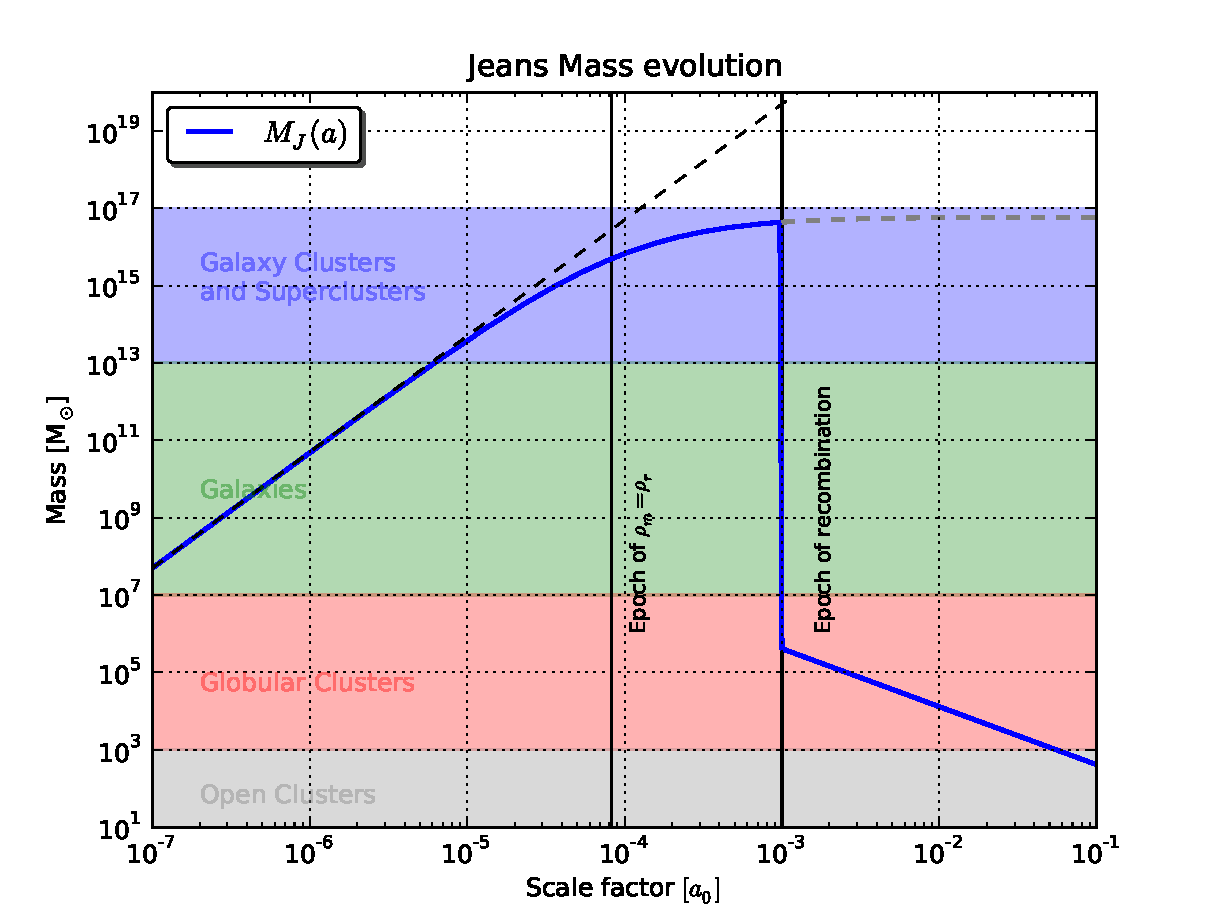
\includegraphics[width=0.9\textwidth]
	{./figures/2_theoretical_framework/Jeans_Mass_Evolution.pdf}

	\caption{\small{Evolution of the Jean mass for different stages of the
	universe. Coloured regions illustrate the typical mass range of some 
	types of structures, since open stellar clusters to superclusters of 
	galaxies.}}
	
	\label{fig:JeansMass}
\end{figure}
%.........................................................................	
	

%Reviewed
The previous analysis has allowed to establish the minimal mass of a 
perturbation in order to collapse. Next it is studied the evolution of 
such perturbations in expanding mediums. For this it is used the models of 
the universe derived in the subsection 
\ref{subsec:SimpleSolutionsOfTheUniverse} and the general equation 
\ref{eq:ContinuityEquationCMode} for evolving perturbations.


\newpage
%.........................................................................
%Solutions to Perturbations Evolution
\begin{itemize}
\item \textbf{Einstein - de Sitter universe}


%Reviewed
Bearing in mind that for this type of universe $\Omega_m = \Omega_0 = 1$, 
using the Hubble's function \ref{eq:EinsteindeSitter}, the solution for 
the scale factor \ref{eq:EinsteindeSitterSolution}, the velocity of sound 
derived from \ref{eq:SoundVelocity} and the equation of state for an ideal 
gas, it leads to the below expression for the evolution of the 
perturbations


%Reviewed
%.........................................................................	
%Einsten-de Sitter Perturbations
\eq{eq:EinstendeSitterPerturbations}
{ \delta_{\bds k}(a) = \delta_{\bds k, 0} \pr{\frac{a}{a_{\submath{ref}}}}^{1} }
%.........................................................................
where $\delta_{\bds k, 0}$ are the conditions of the field over the 
reference time $t_{\submath{ref}}$. Another possible solution is 
$\delta_{\bds k}\propto a^{-3/2}$, but because this solution does not 
decrease over time, it is not interesting.



%Radiation Dominated Universe
\item \textbf{Radiation-dominated universe}


%Reviewed
For perturbations in a radiation-dominated universe with $\Omega_r = 
\Omega_0 = 1$, using the equation \ref{eq:RadiationUniverseSolution}, it
is obtained


%Reviewed
%.........................................................................	
%Radiation Perturbations
\eq{eq:RadiationPerturbations}
{ \delta_{\bds k}(a) = \delta_{\bds k, 0} \pr{\frac{a}{a_{\submath{ref}}}}^{1.22} }
%.........................................................................
where $\delta_{\bds k, 0}$ again represents  the initial modes of the 
field, divergent solutions are ignored.



%Vacuum Dominated Universe
\item \textbf{Vacuum-dominated universe}
			

%Reviewed
For a universe with cosmological constant $\Omega_\Lambda$
\footnote{$\Omega_\Lambda < 1 $ in order to guarantee the convergence of 
solutions to the Friedmann's equation (see subsection 
\ref{subsec:SimpleSolutionsOfTheUniverse}).} it is obtained the next 
behaviour for the evolution of each mode



%.........................................................................	
%Vacuum Perturbations
\eq{eq:VacuumPerturbations}
{ \delta_{\bds k}(a) = \delta_{\bds k, 0} \pr{\frac{a}{a_{\submath{ref}}}}^{0.58} }
%.........................................................................
\end{itemize}
%.........................................................................


%Reviewed
Plotting each one of these solutions, Figure \ref{fig:DeltaEvolution} is 
obtained. For simplicity and in order to illustrate in a better way the 
behaviour of the scale factor, it is normalized each solution with respect
to their respective value in the reference time $\delta_{\bds k, 0}$.


%Reviewed
Initial conditions depend on the comoving wavenumber $\bds k$ and must be
determined from the statistical properties of the density field (see 
subsection \ref{subsec:StatisticalProperties}) and observational 
measurements, for instance the cosmic background radiation.



%Reviewed
%.........................................................................
%Perturbations Evolution
\begin{figure}[htbp]
	\centering
	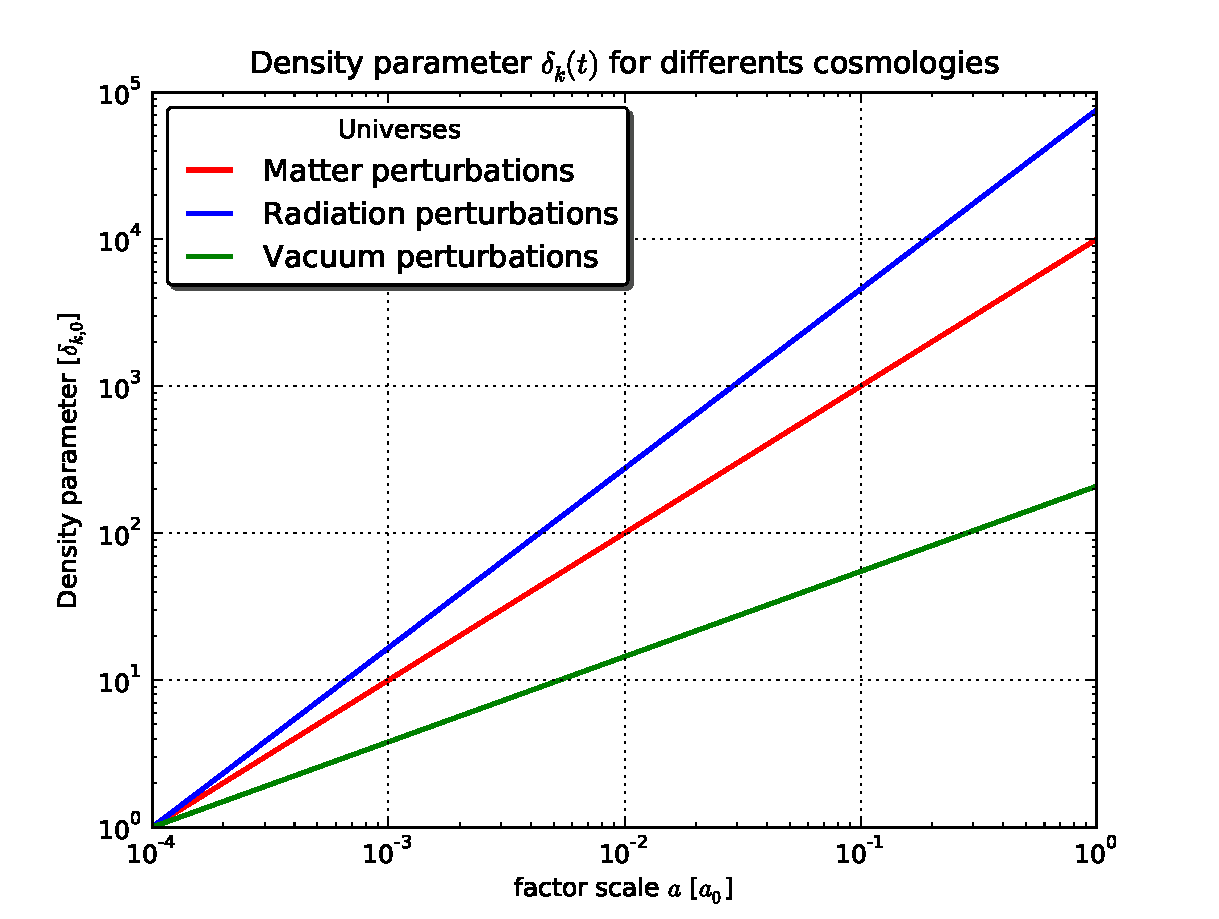
\includegraphics[width=0.9\textwidth]
	{./figures/2_theoretical_framework/Perturbations_Evolution.pdf}

	\caption{\small{Evolution of the normal modes of the density field.
	For the sake of the illustration, each solution has been normalized
	with respect to the initial conditions.}}
	
	\label{fig:DeltaEvolution}
\end{figure}
%.........................................................................	



	%---------------------------------------------------------------------
	%Statistical Properties and Transfer function
	\subsection{Statistical Properties and Transfer Function}
	\label{subsec:StatisticalProperties}
	%---------------------------------------------------------------------


%Reviewed
Once determined how each mode of the density field evolves, it is necessary
to compare this with observations of the real universe. Due to the 
continuous nature of fields, it is infeasible to try to determine 
observationally the density distribution. Moreover, taking into account 
that most of matter is dark, which just can be measured by indirect methods, 
it is technically impossible, with the current instruments, carrying out 
this enterprise.


%Reviewed
In spite of the above, it is still possible to measure the statistical 
properties of the density distribution of the universe and to compare them
with theoretical predictions. In order to do this, it is introduced the 
concept of probability functional of a continuous field 
$P\cor{ \delta(\bds r,t) }$, defined as the probability that a certain 
function has an explicit functional form $\delta(\bds r,t)$.


%Reviewed
A computationally more convenient way to apply the formalism of probability
functional is by discretizing the volume in a set of cells $\Delta^3 \bds 
r_i$, such that a certain explicit functional form of the density field
$\delta(\bds r,t)$ is equivalent to have simultaneously in each cell 
$\bds r_i$ of the grid the value $\delta_i = \delta(\bds r_i)$, so the 
probability functional becomes equal to a joint probability function.



%.........................................................................
%Probability Functional
\eq{eq:ProbabilityFunctional}
{ P\cor{ \delta(\bds r,t)} \ \ \longrightarrow \ \ 
\mathcal{P}_{\bds{r}}(\delta_1,\delta_2,\cdots,\delta_N;t)  }
%.........................................................................


%Reviewed
Taking into account the Fourier decomposition of the density field 
$\delta(\bds r,t)$ introduced in the equations \ref{eq:FourierFields}, it
is possible to define a joint probability function in the reciprocal space
$\mathcal{P}_{\bds k}(\delta_{\bds k_1},\delta_{\bds k_2}, \cdots,
\delta_{\bds k_N};t)$ that completely characterizes the probability of a 
given distribution $\delta_{\bds k}(t)$.


%Reviewed
The main motivation to work over the reciprocal space is because it is 
possible to use the approach of uncorrelated modes, where it is assumed 
that each mode evolves independently of the others. In the real space it
is not possible to assume this since the long-range nature of the 
gravitational interaction couples strongly the density field between 
different locations. A direct consequence of the previous approach is to 
express the joint probability function as the product of $N$ single 
distributions \cite{padmanabhan1995}


%Reviewed
%.........................................................................
%Probability Functional Recipro
\eq{eq:ProbabilityJointFour}
{ \mathcal{P}_{\bds k}(\delta_{\bds k_1},\delta_{\bds k_2},
\cdots,\delta_{\bds k_N};t) = \prod_{\bds k_i}g_{\bds k_i}( \delta_{\bds k_i};t )  }
%.........................................................................
where


%Reviewed
%.........................................................................
%Inverse Fourier Delta
\eq{eq:InverseFourierDelta}
{ \delta_{\bds k} = 
\int_V \delta(\bds r) e^{-i \bds k \cdot \bds r} d^3 \bds r  }
%.........................................................................
$g_{\bds k_i}$ is the single distribution of each mode, $V=L^3$ the 
normalization volume and $\bds k = (2\pi/L)\bds n$, with $\bds n$ a vector
of integer components that characterizes the specific mode.


%Reviewed
Assuming that primordial perturbations of the density field were originated
by the process of cosmic inflation, it is possible to demonstrate that the
distribution of normal modes $g_{\bds k_i}$ is a Gaussian function
\cite{padmanabhan1995}. For convenience, it is decomposed into complex 
polar coordinates the $\delta_{\bds k}$ mode of the density field, 
$\delta_{\bds k} = r_{\bds k}\exp\pr{ i \phi_{\bds k} }$, which leads to 
the next distribution


%Reviewed
%.........................................................................
%Gaussian Distribution
\eq{eq:GaussianDistribution}
{ g_{\bds k}( r_{\bds k}, \phi_{\bds k}; t ) = 
\frac{2(r_{\bds k} dr_{\bds k})}{\sigma_k^2}\pr{ \frac{d\phi_{\bds k}}{2\pi} }
\exp\pr{ -\frac{r_{\bds k}^2}{\sigma_k^2} };\ \ \ \ \ \sigma_k^2 = 2\mu_k^2  }
%.........................................................................
where $\mu_k^2$ is the variance of the distribution and $\sigma_k^2$ is 
the power spectrum. Due to the assumption of isotropy and homogeneity for
the background universe, both quantities only depends on the norm of the 
wave vector $|\bds k| = k$. Furthermore it is direct to demonstrate the 
below properties of the distribution of the field



%.........................................................................
%Distribution Properties
\eq{eq:Distribution Properties}
{ \bra \delta_{\bds k} \ket = 0;\ \ \ \ \ 
  \bra |\delta_{\bds k}|^2 \ket = \sigma_k^2;\ \ \ \ \ 
  \bra \delta_{\bds k} \delta_{\bds p}\ket = 0\ \ \ \mbox{si}\ \ \ \
  \bds k \neq \bds p }
%.........................................................................


%Reviewed
%.........................................................................
%Initial density
\begin{figure}[htbp]
	\centering
	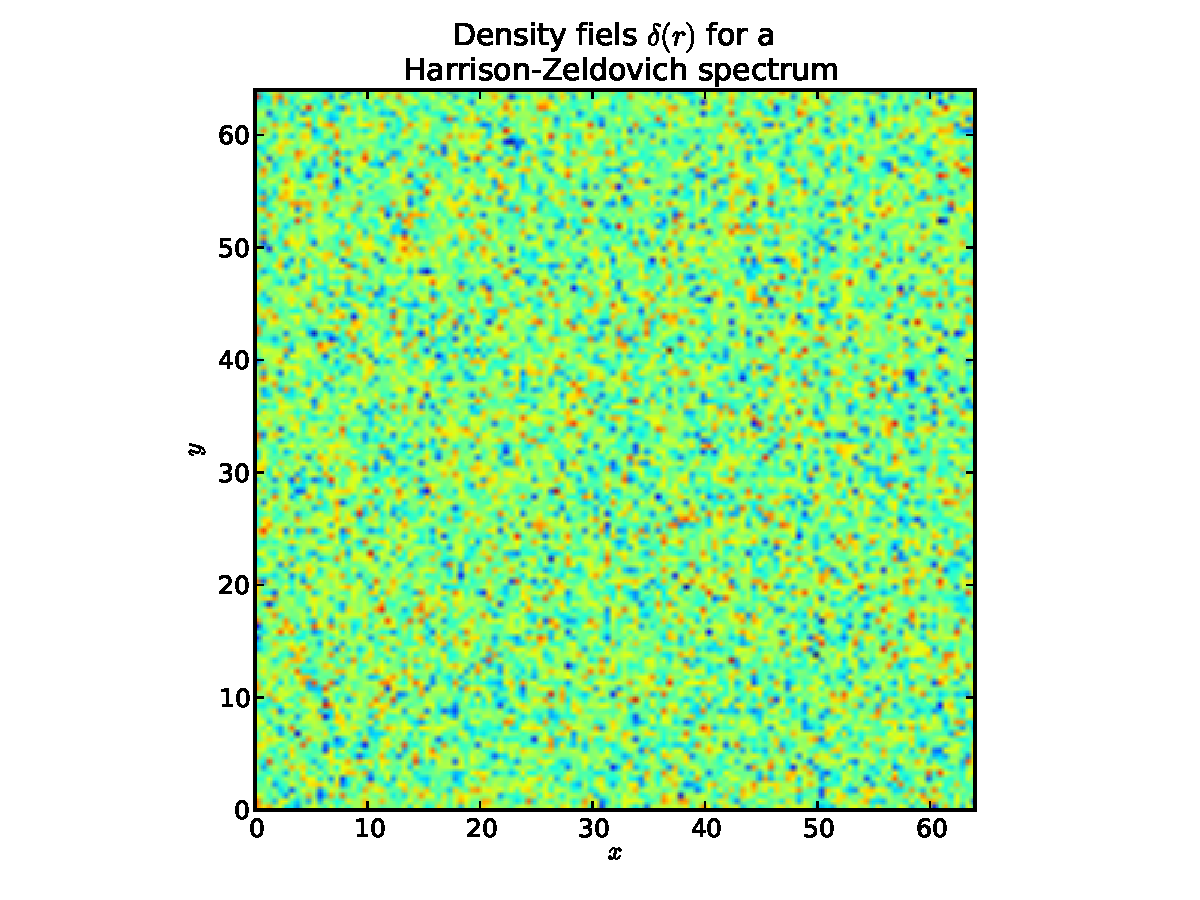
\includegraphics[width=0.8\textwidth]
	{./figures/2_theoretical_framework/Initial_Density.pdf}

	\caption{\small{Initial distribution of perturbations for the density 
	contrast field from the Gaussian distribution 
	\ref{eq:GaussianDistribution} and the Harrison-Zeldovich power spectrum
	$\sigma_k \propto k$.}}	
	\label{fig:InitialDensity}
\end{figure}
%.........................................................................	


%Reviewed
A quantity that can be directly evaluated is the two-point correlation 
function $\xi(\bds r) \equiv \bra \delta(\bds r' + \bds r) \delta(\bds r') 
\ket$, defined as the probability of a perturbation at a distance $\bds r$ 
from another. It is a direct measurement of the anisotropy degree and the 
clustering properties of a certain distribution.


%Reviewed
%.........................................................................
%Two Points Correlation Function
\begin{eqnarray}
\nonumber
\xi(\bds r) = \bra \delta(\bds r' + \bds r) \delta(\bds r') \ket &=& 
\frac{1}{V^2}\sum_{\bds k, \bds p} \bra \delta_{\bds k} \delta_{\bds p}^*\ket
\exp\cor{ i\bds k \cdot(\bds r' + \bds r)- i\bds p \cdot \bds r' } \\
\label{eq:2PCorrelation}
&=& \int \frac{V^{-1}}{(2\pi)^3}\sigma_k^2 e^{i \bds k \cdot \bds r} d^3 \bds k
\end{eqnarray}
%.........................................................................
where in the last line has been performed the continuous approximation. 
The expression \ref{eq:2PCorrelation} shows that $\sigma_k^2$ is the
Fourier transform of the correlation function, that is



%.........................................................................
%Two Points Correlation Function Fourier
\eq{eq:2PCorrelationF}
{ V^{-1}\sigma_k^2 = \int \xi(\bds r) e^{-i\bds k\cdot \bds r}d^3 \bds r }
%.........................................................................


%Reviewed
The previous relation along with the Gaussian distribution of the field 
show that both, the power spectrum and the correlation function, contain
all the statistical information of the density field in the linear regime.
If it is assumed a non-Gaussian distribution, it would be necessary to 
have more moments of the distribution, such as the three-point correlation
function, etc.



			%-------------------------------------------------------------
			%Harrison-Zeldovich Power Spectrum
			\subsubsection*{Harrison-Zeldovich Power Spectrum}
			%-------------------------------------------------------------
			

%Reviewed
A first approximation to the power spectrum of primordial perturbations 
and that can be demonstrated from the model of cosmic inflation
\cite{padmanabhan1995} is the next power law expression


%Reviewed
%.........................................................................
%Power Spectrum power
\eq{eq:PowerSpectrumPower}
{ \sigma_k^2 = A k^{n_s} }
%.........................................................................
where $A$ is a normalization factor and $n$ is the spectral index. In the 
specific case where this index is taken to be $n_s=1$, it is called 
Harrison-Zeldovich power spectrum and is scale invariant \footnote{The 
observed value is very close to 1, $n_s = 0.963$ (see Table
\ref{tab:CosmologicalParameters}).}.


%Reviewed
In order to determine the normalization factor, it is common to apply a
filter to the normal modes that contributes to the density field, which
leads to the next form of the correlation function


%Reviewed
%.........................................................................
%Two Points Correlation Function Fourier with Filter
\eq{eq:Filter2PCorrelation}
{ \xi(\bds r;R) = \int \frac{V^{-1}}{(2\pi)^3}\sigma_k^2 
e^{i \bds k \cdot \bds r} \tilde{W}(k;R) d^3\bds k }
%.........................................................................
where $R$ determines the maximum scale from which is applied the filter
to the modes of the density field and $\tilde{W}(k;R)$ is the Fourier 
transform of the filter function. Specially, it is defined the dispersion
in the real space associated to a scale $R$ as $\sigma^2_R = \bra \delta^2
\ket = \xi(0; R)$, this parameter can be determined observationally from
galaxy surveys and the cosmic background radiation. The value measured by
the WMAP7 release is $\sigma^2_8 = \xi(0; R = 8 \mbox{ Mpc}/h) = 0.801$ 
(see Table \ref{tab:CosmologicalParameters}), this leads to 


%Reviewed
%.........................................................................
%Normalization Expression
\eq{eq:Normalization}
{ \sigma_8^2 = A\int \frac{V^{-1}}{(2\pi)^3} k^{n_s}
 \tilde{W}(k;R=8 \mbox{ Mpc}/h) d^3\bds k }
%.........................................................................
thus, from the measured values of $n_s$ and $\sigma_8^2$, it is possible
to find the correct normalization of the power spectrum.



			%-------------------------------------------------------------
			%Transfer Function
			\subsubsection*{Transfer Function}
			%-------------------------------------------------------------
			

%Reviewed
Finally for the linear regime, it is introduced the concept of transfer 
function $T_{\bds k}(t)$, defined from the below expression


%Reviewed
%.........................................................................
%Transfer function Definition
\eq{eq:TransferFunction}
{ \delta_{\bds k}(t) = T_{\bds k}(t) \delta_{\bds k}(t_i) }
%.........................................................................
where $t_i$ is a reference time, normally taken to be the recombination 
epoch for matter perturbations.


%Reviewed
From the expression \ref{eq:TransferFunction} can be inferred that the 
transfer function contains all the information about the dynamics of the
perturbations, moreover, from the definition \ref{eq:Distribution 
Properties} for the power spectrum it is obtained


%Reviewed
%.........................................................................
%Power Spectrum and Transfer Function
\eq{eq:PkTransferFunction}
{ \sigma_k(t) = \sigma_k(t_i)|T_k(t)|^2 = Ak^{n_s} |T_k(t)|^2 }
%.........................................................................
where it has been assumed a Harrison-Zeldovich power spectrum for the 
reference time. With this, finally it is concluded that the transfer 
function also allows to obtain all the statistical properties of the 
density field during the time when the linear regime is valid.


%Reviewed
Calculating the transfer function is generally a complex process and 
requires numerical computations \footnote{\texttt{CMBFAST} is a 
widely known software for this purpose 
\url{http://lambda.gsfc.nasa.gov/toolbox/tb_cmbfast_ov.cfm}}, 
furthermore, it depends on the specific properties of the specie that 
composes the perturbation. For instance, in the case of dark matter 
perturbations, it must be specified what specific type of particles 
compose the perturbation, either relativistic lightweight particles (hot 
dark matter) or non-relativistic heavy particles (cold dark matter). In
both cases the transfer function and the processed spectrum 
\ref{eq:PkTransferFunction} are quite different due to the equations of
state associated to each type.


%Reviewed
In the case of adiabatic perturbations (isentropic) of cold dark matter,
it can be used the next analytic approximation for the current epoch
\cite{longair2008}


%Reviewed
%.........................................................................
%Transfer Function CDM
\eq{eq:TransferFunctionCDM}
{ T_k \approx \frac{ \ln\pr{ 1 + 2.34 q } }{2.34 q}
\cor{ 1 + 3.89 q + \pr{ 1.61 q }^2 + \pr{ 5.46 q }^3 + \pr{ 6.71 q }^4}^{-1/4} }
%.........................................................................
where $q \equiv k/\Omega_0 h^{2} \mbox{ Mpc}^{-1} $.


%Reviewed
The next Figure illustrates the transfer function 
\ref{eq:TransferFunctionCDM} along with the processed power spectrum


%Reviewed
%.........................................................................
%Transfer Function CDM
\begin{figure}[htbp]
	\centering
	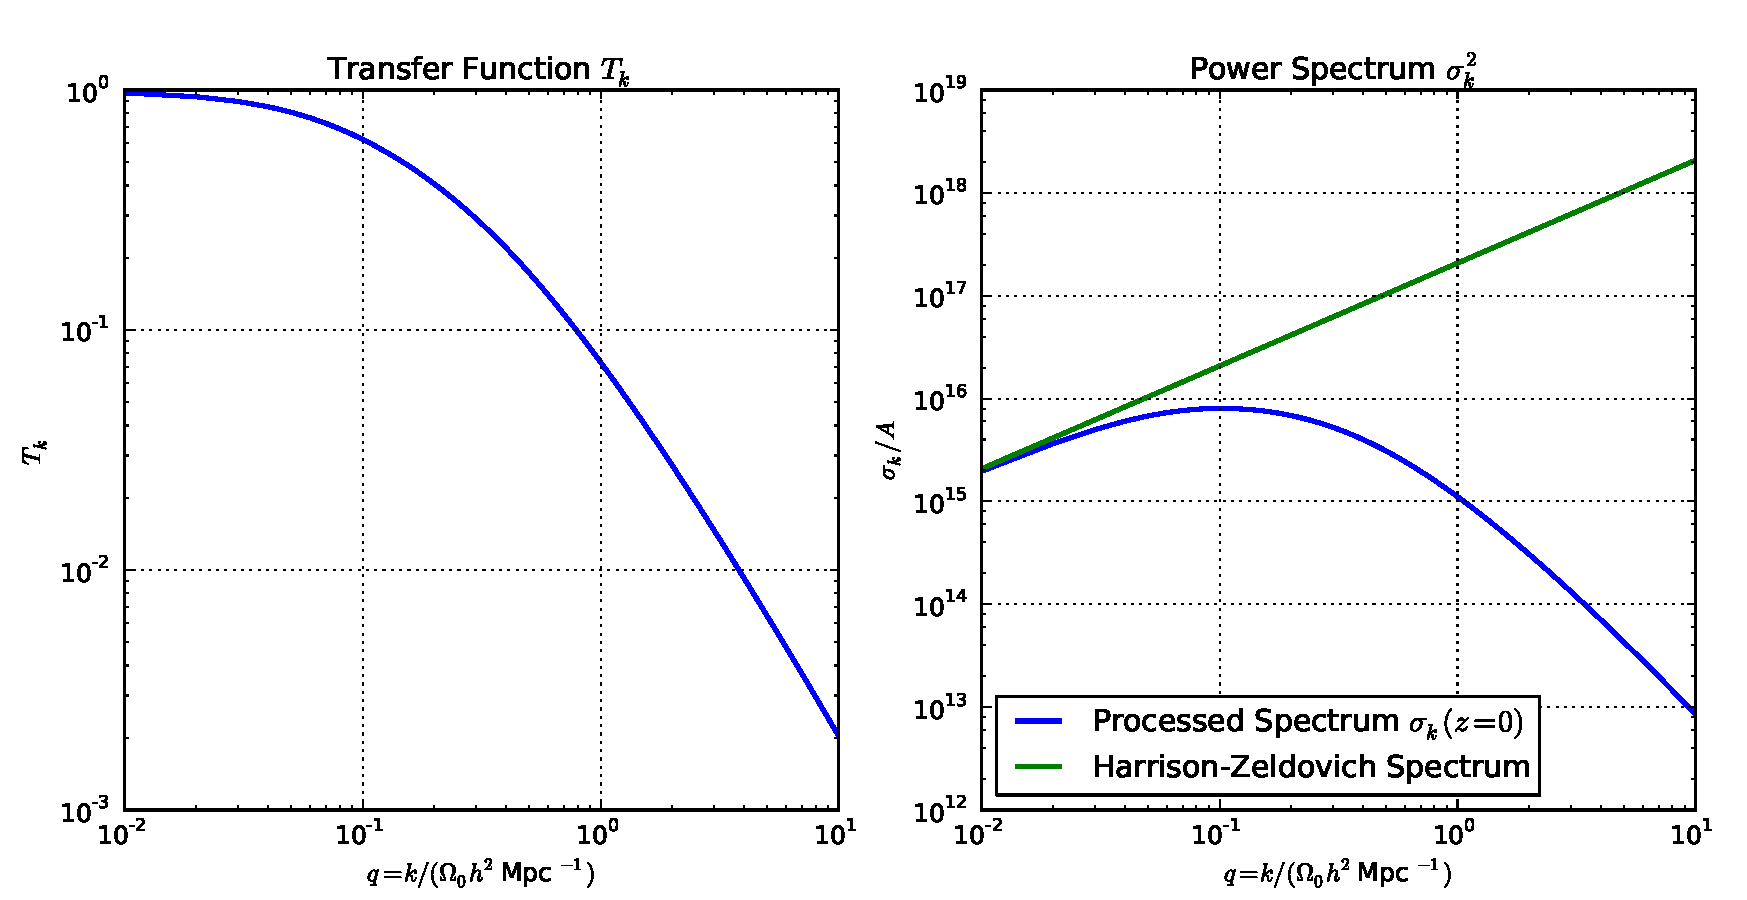
\includegraphics[width=0.9\textwidth]
	{./figures/2_theoretical_framework/Transfer_Function.pdf}

	\caption{\small{Transfer function for cold dark matter perturbations at 
	the current	epoch \cite{longair2008} (left panel). Comparison between 
	the initial	power spectrum, Harrison-Zeldovich spectrum and the processed 
	power spectrum (right panel).}}
	
	\label{fig:TransferFunctionCDM}
\end{figure}
%.........................................................................	


%Reviewed
From all the formalism developed so far in this section, it is concluded 
that the final objective to characterize the linear regime is to obtain 
the transfer function, since it determines completely the evolution of the
universe at early stages, where there were conditions of high isotropy and 
homogeneity at all the scales.



%*************************************************************************




%*************************************************************************
%NonLinear Structure Formation
\section{Non-Linear Regime of Structure Formation}
\label{sec:NonLinearStructureFormation}


%Reviewed
In the linear regime, it is described the process of structure formation
as perturbations within the isotropic and homogeneous background universe.
When perturbations grow up such that $\delta \gtrsim 1$, the self-gravity 
of the modes couples strongly the local density field and invalidates
the linear approximation. The physical processes associated to the 
non-linear regime are highly complex and even some of them are not 
currently well understood, this makes possible to tackle satisfactorily
this problem only through numerical simulations (see chapter
\ref{cha:N-BodySimulations}).


%Reviewed
%.........................................................................
%Nonlinear Universe
\begin{figure}[htbp]
	\centering
	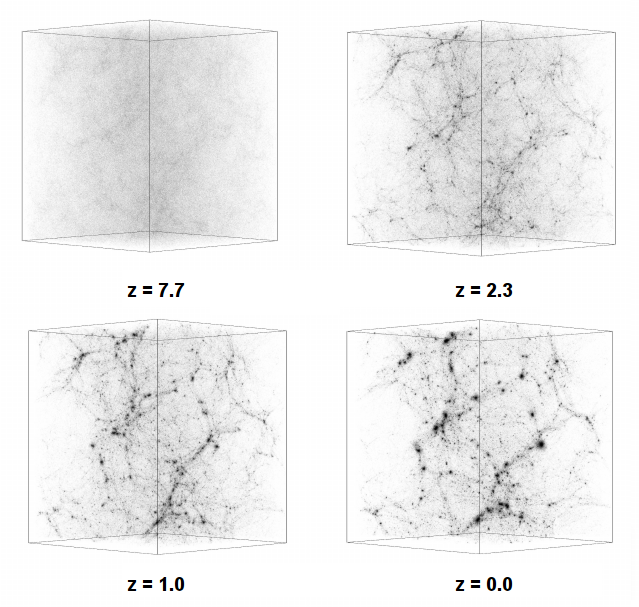
\includegraphics[width=0.9\textwidth]
	{./figures/2_theoretical_framework/Nonlinear.png}

	\caption{\small{Evolution of a dark matter numerical simulation in a 
	comoving volume of $($40 Mpc$/h)^3$, starting from a high homogeneity 
	stage (upper left panel), until the present epoch with highly 
	non-linear structures (lower right panel). Taken from 
	\url{http://www.astro.utu.fi/research/CosmoS/lss/lss_p1.shtml}}}
	
	\label{fig:NonLinearUniverse}
\end{figure}
%.........................................................................


%Reviewed
Figure \ref{fig:NonLinearUniverse} corresponds to different stages of a 
dark matter numerical simulation for the non-linear universe. The Figure 
illustrates some emergent properties such as the anisotropy and 
inhomogeneity at small scales ($\sim$ Mpc), formation and clustering of
highly non-linear structures and the emergence of a web pattern at large
scales (the cosmic web).



	%---------------------------------------------------------------------
	%Zeldovich's Approximation
	\subsection{Zeldovich Approximation}
	\label{subsec:Zeldovich'sApproximation}
	%---------------------------------------------------------------------
	

%Reviewed
In spite of the high complexity of the non-linear regime, when the
perturbations of the density field are not much bigger than the background
value, it is possible to perform an analytic approach to their evolution.
This procedure is called the Zeldovich approximation and was developed by
Yakov Zeldovich in 1970 \cite{zeldovich1970}. In order to formulate this
approximation, it is convenient to express again the contrast density 
field $\delta(\bds r)$ in terms of comoving coordinates instead of Fourier
normal modes. That is because in this regime the Fourier modes are not 
longer independent from each other and using them does not simplify the
problem, unlike the linear regime.


%Reviewed
Using the Lagrangian frame of reference of a certain portion of the fluid,
its trajectory $\bds r_f$ can be described through the next expression


%Reviewed
%.........................................................................
\eq{eq:ZeldovichTrayectory}
{ \bds r_f( t,\bds q ) = a(t)\bds r = a(t)\cor{ \bds q + \bds \Psi(\bds q,t) } }
%.........................................................................
where $\bds r$ is the comoving position of the portion of the fluid, 
$\bds q$ its initial Lagrangian coordinate when the fluid is not perturbed
and $\bds \Psi(\bds q,t)$ is the displacement function that accounts for 
the perturbations of the medium.


%Reviewed
From the equation for the evolution of the contrast density field 
\ref{eq:DeltaEvolution}, it is possible to demonstrate that the 
displacement field $\bds \Psi(\bds q,t)$ satisfies \cite{Yoshisato2006}


%Reviewed
%.........................................................................
%Displacement Differential Equation
\eq{eq:Displacement}
{ \der{^2  \bds \Psi}{t^2} + 2H\der{\bds \Psi}{t} =
 \frac{ 3}{2}H^2 \bds \Psi  }
%.........................................................................
from this, it is finally obtained


%Reviewed
%.........................................................................
%Displacement Explicit Form
\eq{eq:DisplacementForm}
{ \bds \Psi = \frac{3}{2}H_0^{-2}a(t)\nabla \Phi  }
%.........................................................................
where $\Phi$ is the effective gravitational potential associated to the
density field through the Poisson's equation \ref{eq:PoissonEquationC}.


%Reviewed
Rewriting the law of conservation of mass in terms of comoving coordinates
and the initial Lagrangian coordinates, it must be fulfilled


%Reviewed
%.........................................................................
%Mass Conservation
\eq{eq:MassConservation}
{ \rho(\bds r, t)d^3 \bds r = \bar{\rho}(t)d^3 \bds q  }
%.........................................................................
now calculating the Jacobian $\partial q_i / \partial r_j$ of the 
transformation $\bds r \rightarrow \bds q$, the perturbed density field
can be rewritten as \cite{padmanabhan1995}


%Reviewed
%.........................................................................
%Perturbed Field Density
\eq{eq:PerturbedFieldDensity}
{ \rho(\bds r, t) = \frac{\bar \rho (t)}{\pr{ 1 - a(t) \lambda_1(\bds q)}
\pr{ 1 - a(t) \lambda_2(\bds q)}\pr{ 1 - a(t) \lambda_3(\bds q)} } }
%.........................................................................
where $-\lambda_i(\bds q)$ are the eigenvalues of the Jacobian and are 
sorted such that $\lambda_1\geq\lambda_2\geq\lambda_3$. Each one of these
eigenvalues can be interpreted in a geometric way as an indicator of the
collapse or the expansion of a portion of the fluid into the direction
corresponding to the respective eigenvector, thus for example if $\lambda_i 
> 0$, that implies that the density field is collapsing locally into the
direction of the eigenvector $\bds u_i$, whereas if $\lambda_i < 0$ it 
implies an expansion into the same direction.


%Reviewed
%.........................................................................
%Zeldovich Approximation Comparison
\begin{figure}[htbp]
	\centering
	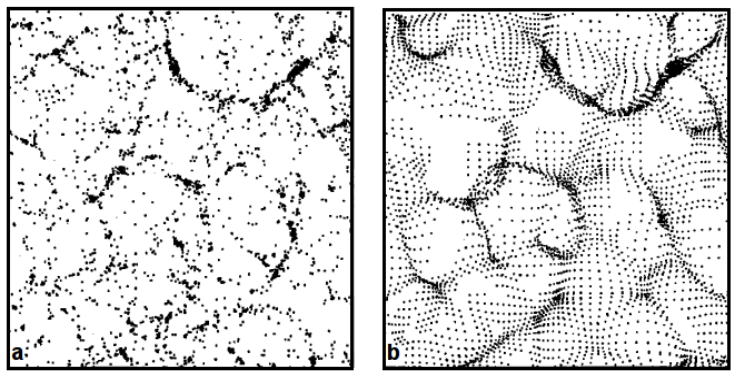
\includegraphics[width=0.9\textwidth]
	{./figures/2_theoretical_framework/Zeldovich_Approximation.png}

	\caption{\small{Comparison of the evolution in non-linear regime
	between a N-body simulation (a) and the Zeldovich approximation (b).
	In both cases are used the same initial conditions. Taken from
	\cite{longair2008}. }}
	
	\label{fig:ZeldovichComparison}
\end{figure}
%.........................................................................


%Reviewed
Finally, Figure \ref{fig:ZeldovichComparison} shows a comparison between a
numerical N-body simulation and the Zeldovich approximation. It can be 
seen a high visual similarity of the obtained structures at the end of the
evolution, thereby showing the high precision of the Zeldovich scheme.
In section \ref{sec:EnvironmentCharacterization} it will be used the
general idea proposed in the Zeldovich approximation regarding the 
eigenvalues of the Jacobian of the transformation, but for building 
classification schemes of the cosmological environment based upon the 
eigenvalues of other physical quantities that are more adequate for 
describing the local dynamics of the density field, such as the tidal 
tensor or the tensor of peculiar velocities.



%*************************************************************************